% По умолчанию используется шрифт 14 размера. Если нужен 12-й шрифт, уберите опцию [14pt]
\documentclass[14pt
  , russian
  %, xcolor={svgnames}
  ]{matmex-diploma-custom}
 
\usepackage[table]{xcolor}
\usepackage{graphicx}
\usepackage{tabularx}
\newcolumntype{Y}{>{\centering\arraybackslash}X}
\usepackage{amsmath}
\usepackage{amsthm}
\usepackage{amsfonts}
\usepackage{amssymb}
\usepackage{mathtools}
\usepackage{thmtools}
\usepackage{thm-restate}
\usepackage{tikz}
\usepackage{wrapfig}
% \usepackage[kpsewhich,newfloat]{minted}
% \usemintedstyle{vs}
\usepackage[inline]{enumitem}
\usepackage{subcaption}
\usepackage{caption}
\usepackage[nocompress]{cite}
\usepackage{makecell}

\usepackage{multirow}
\usepackage{graphicx}
\usepackage{subcaption}
\usepackage{lscape}
\usepackage{longtable}
\usepackage{tikz}
\usepackage{latexsym}

\usepackage{algpseudocode}
\usepackage{algorithm}
\usepackage{algorithmicx}
\usepackage{verbatim}
\usepackage{mathtools}

\usepackage{subcaption}
\usepackage{colortbl}
\usepackage{balance}

% \setitemize{noitemsep,topsep=0pt,parsep=0pt,partopsep=0pt}
% \setenumerate{noitemsep,topsep=0pt,parsep=0pt,partopsep=0pt}


\graphicspath{ {resources/} }

% 
% % \documentclass 
% %   [ a4paper        % (Predefined, but who knows...)
% %   , draft,         % Show bad things.
% %   , 12pt           % Font size.
% %   , pagesize,      % Writes the paper size at special areas in DVI or
% %                    % PDF file. Recommended for use.
% %   , parskip=half   % Paragraphs: noindent + gap.
% %   , numbers=enddot % Pointed numbers.
% %   , BCOR=5mm       % Binding size correction.
% %   , submission
% %   , copyright
% %   , creativecommons 
% %   ]{eptcs}
% % \providecommand{\event}{ML 2018}  % Name of the event you are submitting to
% % \usepackage{breakurl}             % Not needed if you use pdflatex only.
% 
% \usepackage{underscore}           % Only needed if you use pdflatex.
% 
% \usepackage{booktabs}
% \usepackage{amssymb}
% \usepackage{amsmath}
% \usepackage{mathrsfs}
% \usepackage{mathtools}
% \usepackage{multirow}
% \usepackage{indentfirst}
% \usepackage{verbatim}
% \usepackage{amsmath, amssymb}
% \usepackage{graphicx}
% \usepackage{xcolor}
% \usepackage{url}
% \usepackage{stmaryrd}
% \usepackage{xspace}
% \usepackage{comment}
% \usepackage{wrapfig}
% \usepackage[caption=false]{subfig}
% \usepackage{placeins}
% \usepackage{tabularx}
% \usepackage{ragged2e}
% \usepackage{soul}
\usepackage{csquotes}
% \usepackage{inconsolata}
% 
% \usepackage{polyglossia}   % Babel replacement for XeTeX
%   \setdefaultlanguage[spelling=modern]{russian}
%   \setotherlanguage{english}
% \usepackage{fontspec}    % Provides an automatic and unified interface 
%                          % for loading fonts.
% \usepackage{xunicode}    % Generate Unicode chars from accented glyphs.
% \usepackage{xltxtra}     % "Extras" for LaTeX users of XeTeX.
% \usepackage{xecyr}       % Help with Russian.
% 
% %% Fonts
% \defaultfontfeatures{Mapping=tex-text}
% \setmainfont{CMU Serif}
% \setsansfont{CMU Sans Serif}
% \setmonofont{CMU Typewriter Text}

\usepackage[final]{listings}

\lstdefinelanguage{ocaml}{
keywords={@type, function, fun, let, in, match, with, when, class, type,
nonrec, object, method, of, rec, repeat, until, while, not, do, done, as, val, inherit, and,
new, module, sig, deriving, datatype, struct, if, then, else, open, private, virtual, include, success, failure,
lazy, assert, true, false, end},
sensitive=true,
commentstyle=\small\itshape\ttfamily,
keywordstyle=\ttfamily\bfseries, %\underbar,
identifierstyle=\ttfamily,
basewidth={0.5em,0.5em},
columns=fixed,
fontadjust=true,
literate={->}{{$\to$}}3 {===}{{$\equiv$}}1 {=/=}{{$\not\equiv$}}1 {|>}{{$\triangleright$}}3 {\\/}{{$\vee$}}2 {/\\}{{$\wedge$}}2 {>=}{{$\ge$}}1 {<=}{{$\le$}} 1,
morecomment=[s]{(*}{*)}
}

\lstset{
mathescape=true,
%basicstyle=\small,
identifierstyle=\ttfamily,
keywordstyle=\bfseries,
commentstyle=\scriptsize\rmfamily,
basewidth={0.5em,0.5em},
fontadjust=true,
language=ocaml
}
 
\newcommand{\cd}[1]{\texttt{#1}}
\newcommand{\inbr}[1]{\left<#1\right>}


\newcolumntype{L}[1]{>{\raggedright\let\newline\\\arraybackslash\hspace{0pt}}m{#1}}
\newcolumntype{C}[1]{>{\centering\let\newline\\\arraybackslash\hspace{0pt}}m{#1}}
\newcolumntype{R}[1]{>{\raggedleft\let\newline\\\arraybackslash\hspace{0pt}}m{#1}}



\usepackage{soul}
\usepackage[normalem]{ulem}
%\sout{Hello World}



\begin{document}
%% Если что-то забыли, при компиляции будут ошибки Undefined control sequence \my@title@<что забыли>@ru
%% Если англоязычная титульная страница не нужна, то ее можно просто удалить.
\filltitle{ru}{
    %% Актуально только для курсовых/практик. ВКР защищаются не на кафедре а в ГЭК по направлению, 
    %%   и к моменту защиты вы будете уже не в группе.
    chair              = {Кафедра системного программирования},
    group              = {21.М07-мм},
    %% Макрос filltitle ненавидит пустые строки, поэтому обязателен хотя бы символ комментария на строке
    %% Актуально всем.
    title              = {Разработка библиотеки обобщенной разреженной линейной алгебры для вычислений на GPU},
    % 
    %% Здесь указывается тип работы. Возможные значения:
    %%   coursework - отчёт по курсовой работе;
    %%   practice - отчёт по учебной практике;
    %%   prediploma - отчёт по преддипломной практике;
    %%   practice - отчёт по учебной практике;
    %%   master - ВКР магистра;
    %%   bachelor - ВКР бакалавра.
    type               = {master},
    author             = {Орачев Егор Станиславович},
    % 
    %% Актуально только для ВКР. Указывается код и название направления подготовки. Типичные примеры:
    %%   02.03.03 <<Математическое обеспечение и администрирование информационных систем>>
    %%   02.04.03 <<Математическое обеспечение и администрирование информационных систем>>
    %%   09.03.04 <<Программная инженерия>>
    %%   09.04.04 <<Программная инженерия>>
    %% Те, что с 03 в середине --- бакалавриат, с 04 --- магистратура.
    specialty          = {09.04.04 <<Программная инженерия>>},
    % 
    %% Актуально только для ВКР. Указывается шифр и название образовательной программы. Типичные примеры:
    %%   СВ.5006.2017 <<Математическое обеспечение и администрирование информационных систем>>
    %%   СВ.5162.2020 <<Технологии программирования>>
    %%   СВ.5080.2017 <<Программная инженерия>>
    %%   ВМ.5665.2019 <<Математическое обеспечение и администрирование информационных систем>>
    %%   ВМ.5666.2019 <<Программная инженерия>>
    %% Шифр и название программы можно посмотреть в учебном плане, по которому вы учитесь. 
    %% СВ.* --- бакалавриат, ВМ.* --- магистратура. В конце --- год поступления (не обязательно ваш, если вы были в академе/вылетали).
    programme          = {ВМ.5666.2021 <<Программная инженерия>>},
    % 
    %% Актуально только для ВКР, только для матобеса и только 2017-2018 годов поступления. Указывается профиль подготовки, на котором вы учитесь.
    %% Названия профилей можно найти в учебном плане в списке дисциплин по выбору. На каком именно вы, вам должны были сказать после второго курса (можно уточнить в студотделе).
    %% Вот возможные вариканты:
    %%   Математические основы информатики
    %%   Информационные системы и базы данных
    %%   Параллельное программирование
    %%   Системное программирование
    %%   Технология программирования
    %%   Администрирование информационных систем
    %%   Реинжиниринг программного обеспечения
    % profile            = {Системное программирование},
    % 
    %% Актуально всем.
    supervisorPosition = {Доцент кафедры информатики, к.\,ф.-м.\,н.},
    supervisor         = {С.~В.~Григорьев},
    % 
    %% Актуально только для практик и курсовых. Если консультанта нет, закомментировать или удалить вовсе.
    % consultantPosition = {должность ООО <<Место работы>> степень},
    % consultant         = {К.К. Консультант},
    %
    %% Актуально только для ВКР.
    reviewerPosition   = {Эксперт, ООО "Техкомпания Хуавэй"},
    reviewer           = {С.~В.~Моисеев},
}

\filltitle{en}{
    chair              = {Software Engineering},
    group              = {21.М07-мм},
    title              = {Generalized sparse linear algebra library with vendor-agnostic GPUs accelerated computations},
    type               = {master},
    author             = {Egor Orachev},
    % 
    %% Possible choices:
    %%   02.03.03 <<Software and Administration of Information Systems>>
    %%   02.04.03 <<Software and Administration of Information Systems>>
    %%   09.03.04 <<Software Engineering>>
    %%   09.04.04 <<Software Engineering>>
    %% Те, что с 03 в середине --- бакалавриат, с 04 --- магистратура.
    specialty          = {09.04.04 <<Software Engineering>>},
    % 
    %% Possible choices:
    %%   СВ.5006.2017 <<Software and Administration of Information Systems>>
    %%   СВ.5162.2020 <<Programming Technologies>>
    %%   СВ.5080.2017 <<Software Engineering>>
    %%   ВМ.5665.2019 <<Software and Administration of Information Systems>>
    %%   ВМ.5666.2019 <<Software Engineering>>
    programme          = {СВ.5666.2021 <<Software Engineering>>},
    % 
    %% Possible choices:
    %%   Mathematical Foundations of Informatics
    %%   Information Systems and Databases
    %%   Parallel Programming
    %%   System Programming
    %%   Programming Technology
    %%   Information Systems Administration
    %%   Software Reengineering
    % profile            = {Software Engineering},
    % 
    %% Note that common title translations are:
    %%   кандидат наук --- C.Sc. (NOT Ph.D.)
    %%   доктор ... наук --- Sc.D.
    %%   доцент --- docent (NOT assistant/associate prof.)
    %%   профессор --- prof.
    supervisorPosition = {C.Sc., docent},
    supervisor         = {S.~V.~Grigorev},
    % 
    % consultantPosition = {position at ``Company'', degree if present},
    % consultant         = {C.C. Consultant},
    % %
    reviewerPosition   = {Expert, Huawei},
    reviewer           = {S.~V.~Moiseev},
}
\maketitle
\setcounter{tocdepth}{3}
\tableofcontents

% \begin{abstract}
%   В курсаче не нужен
% \end{abstract}

\section*{Введение}

Все чаще современные системы аналитики и рекомендаций строятся на основе анализа данных, структурированных с использованием \textit{графовой модели}. В данной модели основные сущности представляются вершинами графа, а отношения между сущностями --- ориентированными ребрами с различными метками. Подобная модель позволяет относительно легко и практически в явном виде моделировать сложные иерархические структуры, которые не так просто представить, например, в классической \textit{реляционной модели}. В качестве основных областей применения графовой модели можно выделить следующие: графовые базы данных~\cite{article:querying_graph_databases}, анализ RDF данных~\cite{article:cfpq_and_rdf_analysis}, биоинформатика~\cite{article:rna_prediction} и статический анализ кода~\cite{article:dyck_cfl_code_analysis}.

Поскольку графовая модель используется для моделирования отношений между объектами, при решении прикладных задач возникает необходимость в выявлении более сложных взаимоотношений между объектами. Для этого чаще всего формируются запросы в специализированных программных средствах для управления графовыми базами данных. В качестве запроса можно использовать некоторый \textit{шаблон} на путь в графе, который будет связывать объекты, т.е. выражать взаимосвязь между ними. В качестве такого шаблона можно использовать формальные грамматики, например, регулярные или контекстно-свободные (КС). Используя вычислительно более выразительные грамматики, можно формировать более сложные запросы и выявлять нестандартные и скрытые ранее взаимоотношения между объектами. Например, \textit{same-generation queries}~\cite{inbook:databases_intro}, сходные с сбалансированными скобочными последовательностями Дика, могут быть выражены КС грамматиками, в отличие от регулярных.

Результатом запроса может быть множество пар объектов, между которыми существует путь в графе, удовлетворяющий заданным ограничениям. Также может возвращаться один экземпляр такого пути для каждой пары объектов или итератор всех путей, что зависит от семантики запроса. Поскольку один и тот же запрос может иметь разную семантику, требуются различные программные и алгоритмические средства для его выполнения.  

Запросы с регулярными ограничениями изучены достаточно хорошо, языковая и программная поддержка выполнения подобных запросов присутствует в некоторых в современных графовых базах данных. Однако, полноценная поддержка запросов с КС ограничениями до сих пор не представлена. Существуют алгоритмы~\cite{article:cfpq_and_rdf_analysis, article:hellings_cfpq, inproceedings:matrix_cfpq, inbook:kronecker_cfpq_adbis, article:cfpq_go_for_rdf} для вычисления запросов с КС ограничениями, но потребуется еще время, прежде чем появиться полноценная высокпроизводительная реализация одного из алгоритмов, способная обрабатывать реальные графовые данные.

Работы~\cite{inproceedings:cfpq_matrix_evaluation, inproceedings:cfqp_matrix_with_single_source} в качестве реализации алгоритма~\cite{inproceedings:matrix_cfpq} для выполнения запросов с КС ограничениями с семантикой достижимости и семантикой одного пути показывают, что возможно использовать GPGPU для выполнения наиболее вычислительно сложных частей алгоритма, что дает \textit{существенный} прирост в производительности. 

Недавно представленный алгоритм~\cite{inbook:kronecker_cfpq_adbis} для вычисления запросов с КС ограничениями полагается на операции линейной алгебры: произведение Кронекера (частный случай тензорного произведения), умножение и сложение матриц в полукольце булевой алгебры. Важной задачей является реализация данного алгоритма, так как он в сравнении с~\cite{inproceedings:cfqp_matrix_with_single_source} позволяет выполнять запросы для всех ранее упомянутых семантик, потенциально поддерживает б\'ольшие по размеру КС запросы, с незначительными накладными расходами позволяет выполнять запросы с регулярными ограничениями, а с реализацией на GPGPU позволит получить потенциально приемлемое время выполнения запрсов.
\section{Problem statement}

The goal of this work is the implementation of the generalized sparse linear algebra primitives and operations library with portable vendor-agnostic yet high-performance GPUs accelerated computations. The work can be divided into the following tasks.

\begin{itemize}
    \item Conduct the survey of existing solutions, focusing on design principles and programming model, overview technologies and tools for programming GPU computations and highlight challenges of GPU programming.
    
    \item Develop the architecture of the library. Design the high-level library structure, execution model, storage scheme, GPUs backend for vendor-agnostic and portable computations acceleration.
    
    \item Implement the library according to the developed architecture, including library core, backend for GPUs accelerated computations, some GPU optimizations in order to speedup computations, and a set of common graph algorithms.

    % and a high-level package for library distribution.
    
    \item Conduct the preliminary experimental study of implemented artifacts. Analyse the performance of the proposed solution compared to existing tools, test the portability and scalability of the developed library on GPUs of different device vendors.
\end{itemize}
\section{Обзор предметной области}

\subsection{Терминология}

В этой секции изложены основные определения и факты из теории графов и формальных языков, необходимые для понимания предметной области. 
    
\textit{Ориентированный граф с метками} $\mathcal{G} = \langle V, E, L \rangle$ это тройка объектов, где $V$ конечное непустое множество вершин графа, $E \subseteq V \times L \times V$ конечное множество ребер графа, $L$ конечное множество меток графа. Здесь и далее будем считать, что вершины графа индексируются целыми числами, т.е. $V = \{0~...~|V| - 1\}$.

Граф $\mathcal{G} = \langle V, E, L \rangle$ можно представить в виде матрицы смежности $M$ размером $|V| \times |V|$, где $M[i,j] = \{l~|~(i,l,j) \in E\}$. Используя булеву матричную декомпозицию, можно представить матрицу смежности в виде набора матриц $\mathcal{M} = \{ M^l ~|~ l \in L, M^l[i,j] = 1 \iff l \in M[i,l]\}$.

Путь $\pi$ в графе $\mathcal{G} = \langle V, E, L \rangle$ это последовательность ребер $e_0,e_1,e_{n-1}$, где $e_i = (v_i, l_i, u_i) \in E$ и для любых $e_i, e_{i+1}: u_i = v_{i+1}$. Путь между вершинами $v$ и $u$ будем обозначать как $v \pi u$. Слово, которое формирует путь $\pi = (v_0, l_0, v_1), ... ,(v_{n-1}, l_{n-1}, v_n)$ будем обозначать как $\omega (\pi) = l_0 ... l_{n-1}$, что является конкатенацией меток вдоль этого пути $\pi$.

\textit{Контекстно-свободная (КС) грамматика} $G = \langle \Sigma, N, P, S \rangle$ это четверка объектов, где $\Sigma$ конечное множестве терминалов или алфавит, $N$ конечное множество нетерминалов, $P$ конечное множество правил вывода вида $A \rightarrow \gamma, \gamma \in (N \cup \Sigma)^*$, $S \in N$ стартовый нетерминал. 

Язык $L$ над конечным алфавитом символов $\Sigma$ --- множество всевозможных слов, составленных из символов этого алфавита, т.е. $L = \{\omega~|~w \in \Sigma ^*\}$.

\subsection{Поиск путей с ограничениями}

При вычислении запроса $p$ на поиск путей в графе $\mathcal{G} = \langle V, E, L \rangle$ в качестве ограничения выступает некоторый язык $L$, которому должны удовлетворять результирующие пути.

Поиск путей в графе с семантикой \textbf{достижимости}, это поиск всех таких пар вершин $(v,u)$, что между ними существует путь $v \pi u$ такой, что $\omega (\pi) \in L$. Результат запроса обозначается как $R = \{ (v,u)~|~\exists v \pi u : \omega (\pi) \in L \}$.

Поиск путей в графе с семантикой \textbf{всех путей}, это поиск всех таких путей $v \pi u$,   что $\omega (\pi) \in L$. Результат запроса обозначается как $\Pi = \{ v \pi u~|~v \pi u : \omega (\pi) \in L \}$.

Необходимо отметить, что множество $\Pi$ может быть бесконечным, поэтому в качестве результата запроса предполагается не всё множество в явном виде, а некоторый \textit{итератор}, который позволит последовательно извлекать все пути.

Семантика \textbf{одного пути} является ослабленной формулировкой семантики всех путей, так как для получения результата достаточно найти всего один путь вида $v \pi u : \omega (\pi) \in L$ для каждой пары $(v, u) \in R$.

Поскольку язык $L$ может быть бесконечным, при составлении запросов используют не множество $L$ в явном виде, а некоторое правило формирования слов этого языка. В качестве таких правил и выступают регулярные выражения или КС грамматики. При именовании запросов отталкиваются от типа правил, поэтому запросы именуются как регулярные или КС соответственно.

\subsection{Существующие решения}

Впервые проблема выполнения запросов с контекстно-свободными ограничениями была сформулирована в 1990 году в работе Михалиса Яннакакиса~\cite{inproceedings:yannakakis_cfpq_problem}. С того времени были представлены многие работы, в которых так или иначе предлагалось решение данной проблемы. Однако в недавнем исследовании Йохем Куиджперс и др.~\cite{article:kuijpers_cfpq_exp_compare} на основе сравнения нескольких алгоритмов~\cite{article:hellings_cfpq,inproceedings:matrix_cfpq,inbook:santos_cfpq_lr_analysis} для выполнения запросов с контекстно-свободными ограничениями заключили, что существующие алгоритмы неприменимы для анализа реальных данных в силу того, что обработка таких данных занимает значительное время. Стоит отметить, что алгоритмы, используемые в статье, были реализованы на языке программирования \textit{Java} и исполнялись в среде \textit{JVM} в однопоточном режиме, что не является сколь-угодно производительным решением.

Это подтверждают результаты работы~\cite{inproceedings:cfqp_matrix_with_single_source}, в которой с использование программных и аппаратных средств NVIDIA CUDA был реализован алгоритм Рустама Азимова~\cite{inproceedings:matrix_cfpq}. В данном алгоритме задача поиска путей с КС ограничениями для семантики одного пути сведена к операциям линейной алгебры, что позволяет использовать высокопроизводительные библиотеки для выполнения данных операций на GPGPU.

\subsection{Вычисления на GPGPU}

\textit{GPGPU} (от англ. General-purpose computing on graphics processing units) --- техника использования графического процессора видеокарты компьютера для осуществления неспециализированных вычислений, которые обычно проводит центральный процессор. Данная техника позволяет получить значительной прирост производительности, когда необходимо обрабатывать большие массивы данных с фиксированным набором команд по принципу \textit{SIMD}. 

Исторически видеокарты в первую очередь использовались как графические ускорители для создания высококачественной трехмерной графики в режиме реального времени. Однако, позже стало ясно, что мощность графического процессора можно использовать не только для графических вычислений. Так появились программируемые вычислительные блоки (англ. compute shaders), которые позволяют выполнять на видеокарте неграфические вычисления.

На данный момент существует несколько промышленных стандартов программирования вычислений на видеокарте, одними из которых являются Vulkan~\cite{net:spec_vulkan}, OpenGL~\cite{net:spec_opengl}, Direct3D~\cite{net:spec_direct3d} как API для преимущественно графических задач, а также OpenCL~\cite{net:spec_opencl}, NVIDIA CUDA~\cite{net:cuda_toolkit_docs} как API для неспециализированных вычислений.
\section{Библиотека разреженной линейной алгебры на GPGPU}

% Разработка библиотеки \textit{Cubool}~\cite{net:cubool_project}, предоставляющей примитивы линейной булевой алгебры для работы с разреженными данными, осуществляется в рамках исследовательского проекта лаборатории языковых инструментов JetBrains Research.

\subsection{Примитивы и операции}

% Основным примитивом библиотеки является разреженная матрица булевых значений, которая хранится в видеопамяти видеокарты в формате \textit{CSR} (compressed sparse row), который позволяет использовать $O(V + E)$ памяти для хранения матрицы смежности графа. Существуют и другие форматы хранения разреженных матриц: \textit{CSC} (compressed sparse column), \textit{COO} (coordinate list) и так далее. Однако CSR формат был выбран на основе результатов работы~\cite{inproceedings:spgemm_mem_saving_for_nvidia}, так как он позволяет эффективно реализовать операцию матричного умножения в условиях ограниченного объема доступной видеопамяти. 

% В качестве поэлементных операций сложения и умножения используются \textit{логическое-или} и \textit{логическое-и}. Основные функции работы с матрицами для реализации алгоритмов~\cite{inproceedings:matrix_cfpq, inbook:kronecker_cfpq_adbis} представлены ниже:

% \begin{itemize}
%     \item Создание матрицы $M$ размера $m \times n$
%     \item Удаление матрицы $M$ и освобождение занятых ею ресурсов
%     \item Заполнение матрицы $M$ списком значений $(i, j)$, где $i$ и $j$ обозначают строку и столбец ненулевого значения
%     \item Чтение из матрицы $M$ списка значений $(i, j)$, где $i$ и $j$ обозначают строку и столбец ненулевого значения
%     \item Сложение матриц $M + N$
%     \item Умножение матриц $M * N$
%     \item Произведение Кронекера для двух матриц $M \otimes N$
% \end{itemize}

\subsection{Архитектура библитеки}

% Архитектура разработанной библиотеки представлена на рис.~\ref{fig:cubool_architecture}. В качестве языка программирования для написания реализации библиотеки выбран С++, так как он предоставляет механизмы для ручного управления ресурсами, а также позволяет работать с CUDA исполняемым кодом. Исходный код компилируется в разделяемую библиотеку \textbf{libcubool.so}, которая может быть динамически загружена позже в конечное пользовательское приложение. В качестве целевой платформы для исполнения поддерживается семейство операционных систем на базе ядра Linux.

% \begin{figure}[h]
%     \centering
%     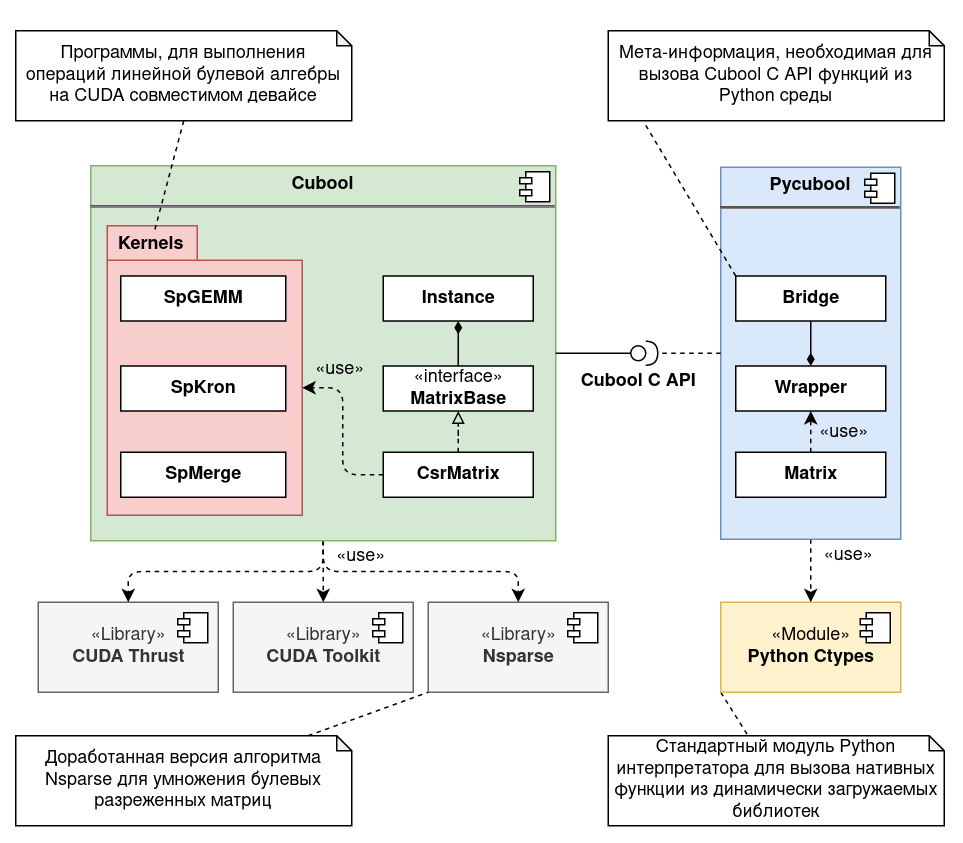
\includegraphics[width=1.0\textwidth]{images/library_architecture.png}
%     \caption{Архитектура разработанной библиотеки}
%     \label{fig:cubool_architecture}
% \end{figure}

\subsection{Детали реализации}

% \subsubsection*{Ядро библиотеки}

% Интерфейс библиотеки написан на языке С, что дает возможность использовать данную библиотеку в С компилируемых приложениях или экспортировать ее функции в среды с управляемыми ресурсами через механизмы исполнения внешнего кода. 

% Реализация библиотеки представлена классом \textbf{Instance}, который поддерживает глобальное состояние и в момент работы предоставляет контекст выполнения для всех операций библиотеки. Класс \textbf{CsrMatrix} представляет разреженную матрицу булевых значений в формате CSR. Данный класс реализует интерфейс \textbf{MatrixBase} и предоставляет доступ ко всем ранее перечисленным операциям.

% Пакет \textbf{Kernels} предоставляет доступ к операциям линейной алгебры, написанным на языке CUDA C++. В качестве основы для реализации операций умножения и сложения матриц использовалась библиотека \textbf{Nsparse}~\cite{inproceedings:cfqp_matrix_with_single_source}, которая была доработана, чтобы добавить возможность динамически конфигурировать механизмы использования видеопамяти. Для реализации произведения Кронекера использовались примитивы библиотеки \textbf{Thrust}, которая позволяет оперировать данными в терминах высокоуровневых операций \textit{свертки}, \textit{отображения} и \textit{префиксной суммы}~\cite{net:cuda_thrust}, которые выполняются на графическом процессоре.     

\subsection{Python-пакет}

% Для работы с примитивами библиотеки на языке Python был разработан модуль \textbf{Pycubool}. Данный инструмент позволит более широкому кругу программистов работать с библиотекой, так как инфраструктура языка Python предоставляет широкий набор утилит для обработки данных, а также поддерживает механизмы автоматического управления ресурсами. Кроме это, использование библиотеки в Python среде позволит переиспользовать существующее решение~\cite{net:cfpq_py_algo} для работы с графовыми данными, которое было получено при реализации алгоритмов~\cite{inbook:kronecker_cfpq_adbis, inproceedings:cfqp_matrix_with_single_source}.

% В качестве инструмента для вызова нативных методов, находящихся в скомпилированной библиотеке libcubool.so, используется модуль \textbf{Ctypes}, так как он поставляется вместе с инфраструктурой Python и не требует настройки сторонних зависимостей. 

% Класс \textbf{Bridge} хранит мета-информацию о методах и примитивах, импортируемых из нативной библиотеки. Класс \textbf{Wrapper} поддерживает глобальное состояние библиотеки и является точкой входа при импортировании модуля \textbf{Pycubool} в исполняемую среду. Класс \textbf{Matrix} предоставляет операции для работы с разреженными матрицами. 

\subsection{Пример использования}

% В качестве примера рассмотрим проблему вычисления \textit{транзитивного замыкания} (англ. transitive closure) для некоторого ориентированного графа без меток $\mathcal{G} = \langle V, E \rangle$. Результатом вычисления транзитивного замыкания является новый граф $\mathcal{G}_{tc} = \langle V, E_{tc} \rangle$, для которого верно следующее: $e = (v,u) \in E_{tc} \iff \exists v \pi u $ в $\mathcal{G}$. Данную проблему можно решить в терминах линейной алгебры, если представить граф в виде матрицы смежности с булевыми значениями. 

% В листинге~\ref{alg:cubool_example} представлен фрагмент кода на языке C, который решает данную задачу. В качестве аргументов функция принимает глобальное состояние библиотеки, матрицу смежности исходного графа, а также указатель на идентификатор, который необходимо использовать при сохранении результирующей матрицы смежности графа после транзитивного замыкания.

% В листинге~\ref{alg:pycubool_example} представлен похожий фрагмент кода, однако он уже решает поставленную в задачу на языке Python. Здесь в качестве входного аргумента используется матрица смежности графа, в качестве результата возвращается матрица смежности графа после транзитивного замыкания. Передача состояния библиотеки здесь не требуется, так как оно неявно передается во все вызовы нативных методов. 

% \definecolor{codegreen}{rgb}{0,0.6,0}
% \definecolor{codegray}{rgb}{0.5,0.5,0.5}
% \definecolor{codepurple}{rgb}{0.58,0,0.82}
% \definecolor{backcolour}{rgb}{1.0,1.0,1.0}

% \lstdefinestyle{codelistingstyle}{
%     backgroundcolor=\color{backcolour},   
%     commentstyle=\color{codegreen},
%     keywordstyle=\color{magenta},
%     numberstyle=\tiny\color{codegray},
%     stringstyle=\color{codepurple},
%     basicstyle=\ttfamily\footnotesize,
%     breakatwhitespace=false,         
%     breaklines=true,                 
%     captionpos=b,                    
%     keepspaces=true,                 
%     numbers=left,                    
%     numbersep=5pt,                  
%     showspaces=false,                
%     showstringspaces=false,
%     showtabs=false,                  
%     tabsize=2
% }

% \lstset{style=codelistingstyle}

% \begin{algorithm}[h]
% \floatname{algorithm}{Listing}
% \caption{Пример вычисления транзитивного замыкания с использованием Cubool C API}
% \label{alg:cubool_example}
% \begin{lstlisting}[language=C++]
% CuBoolStatus TransitiveClosure(CuBoolInstance Inst, CuBoolMatrix A, CuBoolMatrix* T) {
%     CuBool_Matrix_Duplicate(Inst, A, T);         /** Копируем матрицу смежности А */

%     CuBoolSize_t total = 0;
%     CuBoolSize_t current;
%     CuBool_Matrix_Nvals(Inst, *T, &current);     /** Количество ненулевых значений */

%     while (current != total) {                   /** Пока результат меняется  */
%         total = current;
%         CuBool_MxM(Inst, *T, *T, *T);            /** T += T * T */
%         CuBool_Matrix_Nvals(Inst, *T, &current);
%     }

%     return CUBOOL_STATUS_SUCCESS;
% }
% \end{lstlisting}
% \end{algorithm}

% \begin{algorithm}[h]
% \floatname{algorithm}{Listing}
% \caption{Пример вычисления транзитивного замыкания с использованием Pycubool}
% \label{alg:pycubool_example}
% \begin{lstlisting}[language=Python]
% def transitive_closure(a: pycubool.Matrix):
%     t = a.duplicate()                 # Копируем матрицу смежности А
%     total = 0                         # Количество ненулевых значений результата

%     while total != t.nvals:           # Пока результат меняется
%         total = t.nvals
%         pycubool.mxm(t, t, t)         # t += t * t

%     return t
% \end{lstlisting}
% \end{algorithm}
\section{Текущий прогресс}

Прогресс в работе на данный момент:

\begin{itemize}
    \item Выбран технологический стек для реализации библиотеки матричных примитивов: С/C++ для реализации интерфейса библиотеки и ее функциональности, CMake для сборки проекта, NVIDIA CUDA Toolkit 10 для написания кода, исполняемого на CUDA-совместимой видеокарте, NVIDIA Thrust для автоматизации работы с неуправляемыми ресурсами GPU
    \item Создан репозиторий проекта~\cite{net:cubool_project}, настроена автоматическая сборка с использованием инструментария \textit{Github Actions}. Добавлено описание проекта и инструкция для сборки.
    \item Создан C совместимый интерфейс для работы с примитивами библиотеки, а также добавлена непосредственно реализация интерфейса: создание и удаление матриц, запись и чтение значений матрицы, операции умножения, сложения, произведение Кронекера.
    \item Добавлен набор \textit{unit}-тестов для проверки корректности работы операций на основе сравнения с эталонной реализации тестируемых операций на ЦПУ.
    \item На языке Python с использованием библиотеки Ctypes реализован базовый уровень абстракции, необходимый для использования функции библиотеки матричных операций в тестовой инфраструктуре, которая также реализована на языке Python. Выбор Ctypes обусловлен тем, что данный модуль включен в стандартную поставку Python интерпретатора.
\end{itemize}

% \section{Эксперимент}
% Как мы проверяем, что  всё удачно получилось

% \subsection{Условия эксперимента}
% Железо (если актуально); входные данные, на которых проверяем наш подход; почему мы выбрали именно эти тесты

% \subsection{Исследовательские вопросы (Research questions)}
% Надо сформулировать то, чего мы хотели бы добиться работой (2 штуки будет хорошо):

% \begin{itemize}
% \item Хотим алгоритм, который лучше вот таких-то остальных
% \item Если в подходе можно включать/выключать составляющие, то насколько существенно каждая составляющая влияет на улучшения
% \item Если у нас строится приближение каких-то штук, то на сколько точными будут эти приближения
% \item и т.п.
% \end{itemize}

% \subsection{Метрики}

% Как мы сравниваем, что результаты двух подходов лучше или хуже
% \begin{itemize}
% \item Производительность
% \item Строчки кода
% \item Как часто алгоритм "угадывает" правильную классификацию входа
% \end{itemize}

% Иногда метрики вырожденные (да/нет), это не очень хорошо, но если в области исследований так принято, то ладно.

% \subsection{Результаты}
% Результаты понятно что такое. Тут всякие таблицы и графики

% В этом разделе надо также коснуться Research Questions.

% \subsubsection{RQ1} Пояснения
% \subsubsection{RQ2} Пояснения

% \subsection{Обсуждение результатов}

% Чуть более неформальное обсуждение, то, что сделано. Например, почему метод работает лучше остальных? Или, что делать со случаями, когда метод классифицирует вход некорректно.

% \section{Применение того, что сделано на практике (опциональный)}

% Если применение в лоб не работает, потому что всё изложено чуть более сжато и теоретично, надо рассказать тонкости и правильный метод применения результатов. 

% \section{Угрозы нарушения корректности (опциональный)}

% Если основная заслуга метода, это то, что он дает лучшие цифры, то стоит сказать, где мы могли облажаться, когда проводили численные замеры. 

% \section{Заключение}

% Кратко, что было сделано. Также здесь стоит писать задачи на будущее.

% \textbf{Для курсовых/дипломов.} Также стоит сделать список результатов, который будет 1 к одному соответствовать задачам из раздела~\ref{sec:task}.

% \begin{itemize}
% \item Результат к задаче 1 
% \item Результат к задаче 2
% \item и т.д.
% \end{itemize}

% \nocite{*}
\setmonofont[Mapping=tex-text]{CMU Typewriter Text}
\bibliographystyle{ugost2008ls}
\bibliography{kronecker_cfpq_gpu}

\end{document}